\subsection{Đề 2}
	\Opensolutionfile{ans}[ans/2GKII-DE2-1]
\caulc

\begin{ex}%[2D4N1-2]
	Tìm họ nguyên hàm của hàm số $f(x)=3 x^2+1$.
	\choice
	{$x^3+C$}
	{$\dfrac{x^3}{3}+x+C$}
	{\True $x^3+x+C$}
	{$6 x+C$}
	\loigiai{
		Ta có
		\begin{eqnarray*}
			\displaystyle\int f(x) \mathrm{\,d}x&=&\displaystyle\int \left( 3 x^2+1 \right) \mathrm{\,d}x\\
			&=&x^3+x+C.
		\end{eqnarray*}
	}
\end{ex}

\begin{ex}%[2D4H1-3]
	Cho hàm số $y=f(x)$ có đạo hàm trên $\mathbb{R}$ thỏa mãn $f'(x)=3-5\sin x$ và $f(0)=14$. Trong các khẳng định sau, khẳng định nào đúng?
	\choice
	{$f(x)=3x-5\cos x+9$}
	{$f(x)=3x-5\sin x+14$}
	{\True $f(x)=3x+5\cos x+9$}
	{$f(x)=3x+5\sin x+14$}
	\loigiai{
		Ta có $(x)=\displaystyle\int(3-5\sin x)\mathrm{\,d}x=3x+5\cos x+C$.\\
		Với $f(0)=14\Leftrightarrow 5+C=14\Leftrightarrow C=9$.\\
		Vậy $f(x)=3x+5\cos x+9$.
	}
\end{ex}

\begin{ex}%[2D4N2-1]
	Biết $\displaystyle \int\limits_1^3 f(x)\mathrm{\,d}x=2$. Giá trị của $\displaystyle \int\limits_1^3 3f(x)\mathrm{\,d}x$ bằng
	\choice
	{$5$}
	{\True $6$}
	{$\dfrac{2}{3}$}
	{$8$}
	\loigiai
	{
		Ta có $\displaystyle \int\limits_1^3 3f(x)\mathrm{\,d}x=3 \int\limits_1^3 f(x)\mathrm{\,d}x=3\cdot 2=6$.
	}
\end{ex}


\begin{ex}%[2D4N2-2]
	Cho $\displaystyle \int \limits_{0}^{1}f(x)\mathrm{d}x=4$, khi đó $\displaystyle \int \limits_{0}^{1}[f(x)+2x]\mathrm{d}x$ bằng
	\choice
	{$6$}
	{$3$}
	{$2$}
	{\True $5$}
	\loigiai{
		Ta có $\displaystyle \int \limits_{0}^{1}[f(x)+2x]\mathrm{d}x=\int \limits_{0}^{1}f(x)\mathrm{d}x+\int \limits_{0}^{1} 2x\mathrm{d}x=4 + 1 = 5$.
	}
\end{ex}

\begin{ex}%[2D4N3-1]
	\immini{
		Cho hàm số $ y=f\left(x\right)$ liên tục trên $\left[-2;3\right]$ và có đồ thị như hình vẽ. Biết $\displaystyle\int\limits_{-2}^0f\left(x\right)\mathrm{\, d}x=a$, $\displaystyle\int\limits_0^3f\left(x\right)\mathrm{\, d}x=b$. Tính diện tích của phần được gạch chéo theo $ a$, $ b$.
		\choice
		{$ a+b$}
		{$ b-a$}
		{$\dfrac{a+b}{2}$}
		{\True $ a-b$}
	}{
		\begin{tikzpicture}[line join=round, line cap=round,>=stealth,scale=0.5]
			\def\xmin{-3}\def\xmax{4}\def\ymin{-3}\def\ymax{3}
			\draw[->] (\xmin-0.2,0)--(\xmax+0.2,0) node[below] {\footnotesize $x$};
			\draw[->] (0,\ymin-0.2)--(0,\ymax+0.2) node[right] {\footnotesize $y$};
			\draw (0,0) node [below left] {\footnotesize $O$};
			\foreach \x in {-2,3}\draw (\x,0.1)--(\x,-0.1) node [above left] {\footnotesize $\x$};
			\clip (\xmin,\ymin) rectangle (\xmax,\ymax);
			\draw[line width=0.8pt,smooth,samples=200,domain=\xmin:\xmax] plot (\x,{(1*((\x)^3)+-1*((\x)^2)+-6*(\x)+0)/3});
			\draw[pattern = north east lines, domain=-2:0,line width = 0.5pt,samples=100] (-2,0) plot(\x, {(1*((\x)^3)+-1*((\x)^2)+-6*(\x)+0)/3})--(0,0);
			\draw[pattern = north east lines, domain=0:3,line width = 0.5pt,samples=100] (0,0) plot(\x, {(1*((\x)^3)+-1*((\x)^2)+-6*(\x)+0)/3})--(3,0);
			\filldraw (-2,0) circle (2pt);
			\filldraw (0,0) circle (2pt);
			\filldraw (3,0) circle (2pt);
		\end{tikzpicture}
	}
	\loigiai{
		Diện tích $ S$ của phần bị gạch chéo là
		$$ S=\displaystyle\int\limits_{-2}^0f\left(x\right)\mathrm{\, d}x-\displaystyle\int\limits_0^3 f\left(x\right)\mathrm{\, d}x=a-b.$$
	}
\end{ex}

\begin{ex}%[2D4H3-4]
	Trong không gian, xét một vật thể được giới hạn bởi hai mặt phẳng $x=1$ và $x=5$. Nếu cắt vật thể bằng một mặt phẳng vuông góc với trục $Ox$ tại điểm có hoành độ $x$ $(1\le x\le 5)$ thì thiết diện thu được là tam giác đều có cạnh bằng $\dfrac{2}{3}x$. Thể tích của vật thể đó bằng
	\choice
	{$\dfrac{124}{27}$}
	{\True $\dfrac{124\sqrt{3}}{27}$}
	{$\dfrac{248\sqrt{3}}{27}\pi$}
	{$\dfrac{124\sqrt{3}}{27}\pi$}
	\loigiai{
		Ta có $V=\displaystyle\int\limits_1^5 \left(\dfrac{2}{3}x\right)^2 \cdot\dfrac{\sqrt{3}}{4} \mathrm{\,d}x=\displaystyle\int\limits_1^5 \dfrac{\sqrt{3}}{9}x^2 \mathrm{\,d}x=\dfrac{\sqrt{3}}{27}x^3\bigg|_1^5=\dfrac{124\sqrt{3}}{27}$.
	}
\end{ex}

\begin{ex}%[2H5N1-3]
	Trong không gian $Oxyz$, mặt phẳng $(Oyz)$ có phương trình là
	\choice
	{$y=0$}
	{\True $x=0$}
	{$x+y+z=0$}
	{$z=0$}
	\loigiai{
		Phương trình mặt phẳng $(Oyz)$ là $x=0$.
	}
\end{ex}

\begin{ex}%[2H5H1-4]
	Trong không gian $Oxyz$ cho hai mặt phẳng $ (P)\colon -6x+my-2mz-m^{2}=0 $ và $ (Q)\colon 2x+y-2z+3=0 $ ($m$ là tham số). Tìm $m$ để mặt phẳng $(P)$ vuông góc với mặt phẳng $(Q)$.
	\choice
	{\True $ m=\dfrac{12}{5} $}
	{$ m=12 $}
	{$ m=\dfrac{12}{7} $}
	{$ m=\dfrac{5}{12} $}
	\loigiai{
		Véc-tơ pháp tuyến của $(P)$ là $ \vec{n}_{P}=(-6;m;-2m)$, véc-tơ pháp tuyến của $ (Q) $ là $ \vec{n}_{Q}=(2;1;-2) $.\\
		Mặt phẳng $(P)$ vuông góc với mặt phẳng $(Q)$ khi và chỉ khi
		\[
		\vec{n}_{P}\cdot\vec{n}_{Q}=0\Leftrightarrow -12+m+4m=0\Leftrightarrow m=\dfrac{12}{5}.
		\]
	}
\end{ex}

\begin{ex}%[2H5H1-3]
	Trong không gian $Oxyz$, cho tam giác $ABC$ với $A\left(1;1;-2 \right) $, $B\left( 2;0;3\right) $, $C(-2;4;1)$. Mặt phẳng
	$(ABC)$ có phương trình là
	\choice
	{$x+y-z+2=0$}
	{$x+y-2z+2=0$}
	{\True $x+y-2=0$}
	{$x+y+z-2=0$}
	\loigiai{
		Hai véc-tơ không cùng phương có giá song song hoặc nằm trên $(ABC)$ là
		\[\vec{AB}=(1;-1;5)\ \text{và}\ \vec{AC}=(-3;3;3).\]
		Do đó mặt phẳng $(ABC)$ có véc-tơ pháp tuyến là
		\[\vec{n}=\left[\vec{AB},\vec{AC} \right]=(-18;-18;0).\]
		Vậy phương trình của $(ABC)$ là
		\[-18(x-1)-18(y-1)+0(z+2)=0\Leftrightarrow x+y-2=0.\]
	}
\end{ex}

\begin{ex}%[2H5N2-3]
	Trong không gian $Oxyz$, phương trình của trục tung $Oy$ là
	\choice
	{$\heva{&x=0\\ & y=t\\ & z=t}$}
	{$\heva{&x=t\\ & y=t\\ & z=0}$}
	{$\heva{&x=t\\ & y=0\\ & z=t}$}
	{\True $\heva{&x=0\\ & y=t\\ & z=0}$}
	\loigiai{
	}
\end{ex}

\begin{ex}%[2H5H2-3]
	Trong không gian $Oxyz$, đường thẳng đi qua hai điểm $A(1; 2;-1)$ và $B(2;-1; 1)$ có phương trình tham số là
	\choice
	{$\heva{&x=1+t\\& y=-3+2t\\& z=2-t}$}
	{\True $\heva{&x=1+t\\& y=2-3t\\& z=-1+2 t}$}
	{$\heva{&x=1+t\\& y=1+2t \\& z=-t}$}
	{$\heva{&x=1+t\\&y=2-3t\\&z=1+2t}$}
	\loigiai{
	Ta có $\vec{AB}=(1;-3;2)$ là véc-tơ chỉ phương của đường thẳng $AB$.\\
	Mặt khác đường thẳng $AB$ đi qua điểm $A(1;2;-1)$ nên có phương trình tham số là
		$\left\{\begin{aligned}
			&x=1+t\\
			&y=2-3t\\
			&z=-1+2t\\
		\end{aligned}\right.,\,t\in \mathbb{R}.$
	}
\end{ex}


\begin{ex}%[2H5H2-7]
	Trong không gian $Oxyz$, cho đường thẳng $\Delta\colon\dfrac{x-1}{1}=\dfrac{y-2}{2}=\dfrac{z}{-2}$ và mặt phẳng $(P)\colon 2x-y+2z-3=0 $. Gọi $\alpha $ là góc giữa đường thẳng $\Delta $ và mặt phẳng $(P)$. Khẳng định nào sau đây là đúng?
	\choice
	{\True $\sin\alpha=\dfrac{4}{9}$}
	{$\cos\alpha=-\dfrac{4}{9}$}
	{$\sin\alpha=-\dfrac{4}{9}$}
	{$\cos\alpha=\dfrac{4}{9}$}
	\loigiai{
		Đường thẳng $\Delta $ có vtcp $\vec{u}=(1; 2;-2)$, mặt phẳng $(P)$ có vtpt $\vec{n}=(2;-1; 2)$.\\
		Khi đó $$\sin\alpha=\dfrac{\left|\vec{u}\cdot\vec{n}\right|}{\left|\vec{u}\right|\cdot\left|\vec{n}\right|}=\dfrac{\left|2-2-4\right|}{\sqrt{1+4+4}\cdot\sqrt{4+1+4}}=\dfrac{4}{9}.$$
	}
\end{ex}

\Closesolutionfile{ans}
\indapan{6}{ans/2GKII-DE2-1}

\cauds
\Opensolutionfile{ans}[ans/2GKII-DE2-2]

\begin{ex}%[2D4N2-1]
	Cho $f(x)$ là hàm số liên tục trên đoạn $[a ; b]$. Giả sử $F(x)$ và $G(x)$ là hai nguyên hàm của $f(x)$ trên đoạn $[a ; b]$.
	\choiceTF
	{\True $G(x)=F(x)+C$, với $C$ là hằng số nào đó}
	{$\displaystyle\int\limits_{a}^{b} f(x)\mathrm{\,d}x=G(b)-F(a)$}
	{\True $\displaystyle\int\limits_{a}^{b} f(x)\mathrm{\,d}x=F(b)-F(a)$}
	{\True $F(b)+G(a)=G(b)+F(a)$}
	\loigiai{
		\begin{itemchoice}
			\itemch Theo định lý thì $F(x)$ và $G(x)$ là hai nguyên hàm của $f(x)$ trên đoạn $[a ; b]$ thì $G(x)=F(x)+C$, với $C$ là hằng số nào đó.
			\itemch $\displaystyle\int\limits_{a}^{b} f(x)\mathrm{\,d}x=G(x)\Big|_a^b=G(b)-G(a)$\quad (1).
			\itemch $\displaystyle\int\limits_{a}^{b} f(x)\mathrm{\,d}x=F(x)\Big|_a^b=F(b)-F(a)$ \quad (2).
			\itemch Từ (1) và (2), suy ra $G(b)-G(a)=F(b)-F(a) \Leftrightarrow F(b)+G(a)=G(b)+F(a)$.
		\end{itemchoice}
	}
\end{ex}

\begin{ex}%[2D4V3-3]
	\immini{Cho $y=f(x)$ là hàm số bậc hai có đồ thị $(P)$ như hình vẽ bên. Gọi $(H)$ là hình phẳng giới hạn bởi $(P)$ với trục hoành.
		\choiceTF
		{Hoành độ giao điểm của parabol với trục hoành là $x=1$ và $x=2$}
		{\True Phương trình của parabol là $y=2x-x^2$}
		{Diện tích của hình $(H)$ bằng $\dfrac{2}{3}$}
		{Khi cho hình $(H)$ xoay quanh trục $Ox$ ta được một vật thể có thể tích bằng $\dfrac{16}{15}$}
	}
	{\hspace{1cm}
		\begin{tikzpicture}[>= stealth,font=\scriptsize,line width=1.2pt,line cap =round, line join = round,scale=1.3]
			\def\a{1}
			\def\f(#1){2*(#1)-(#1)^2}
			\pgfmathsetmacro\fa{\f(\a)}
			\fill[pattern=north east lines] plot[domain=0:2] (\x,{\f(\x)}) -- (0,0) -- cycle;
			\draw[->] (-0.5,0) -- (3,0) node[below]{$x$};
			\draw[->] (0,-1) -- (0,1.5) node[right]{$y$};
			\draw (0,0) node[below left] {$O$} (2,0) node[above right] {$2$} ;
			\draw[smooth,domain=-0.3:2.2,samples=100] plot (\x,{\f(\x)}) node[below] {$y=f(x)$};
			\draw[dashed] (0,1)node[left] {$1$} -- (1,1)--(1,0)node[below] {$1$} ;
	\end{tikzpicture}}
	\loigiai{	
		\begin{itemchoice}
			\itemch Từ hình vẽ ta thấy đồ thị cắt trục hoành tịa hai điểm có hoành độ lần lượt là $x=0$ và $x=2$.
			\itemch Tọa độ đỉnh của $(P)$ là $(1;1)$ nên phương trình parabol có dạng $y=a(x-1)^2+1$.\\
			Mặt khác $(P)$ qua $(0;0)$, suy ra $a(0-1)^2+1=0 \Rightarrow a=-1$.\\ 
			Vậy $y=-1(x-1)^2+1=2x-x^2$.
			\itemch Diện tích hình $(H)$ là $S=\displaystyle\int\limits_0^2 \left(2x-x^2\right) \mathrm{\, d}x=\dfrac{2}{3}$.
			\itemch Thể tích được tính bởi công thức $V=\pi\displaystyle\int\limits_0^2 \left(2x-x^2\right)^2 \mathrm{\, d}x=\dfrac{16}{15}\pi$.
		\end{itemchoice}
	}
\end{ex}

\begin{ex}%[2H5H1-6]
	Trong không gian $Oxyz$, cho mặt phẳng $(P)\colon x+y+z-3=0$ và mặt phẳng $(Q) \colon x-2y+z=0$
	\choiceTF
	{\True $\vec{n}=(1;1;1)$ là một véc-tơ pháp tuyến của mặt phẳng $(P)$}
	{Điểm $A(1;0;3)$ thuộc mặt phẳng $(Q)$}
	{Khoảng cách từ điểm $B(1;2;3)$ đến mặt phẳng $(P)$ bằng $\sqrt{2}$}
	{\True Góc giữa mặt phẳng $(P)$ và mặt phẳng $(Q)$ bằng $90^\circ$}
	\loigiai
	{
		\begin{itemchoice}
			\itemch $\vec{n}=(1;1;1)$ là một véc-tơ pháp tuyến của $(P)$.
			\itemch Thay toạ độ điểm $A$ vào phương trình mặt phẳng $(Q)$ thấy không thoả mãn. Do đó  điểm $A$ không thuộc mặt phẳng $(Q)$.
			\itemch $\mathrm{d}(B;(P))=\dfrac{\left|1+2+3-3 \right|}{\sqrt{1^2+1^2+1^2}}=\sqrt{3}$.
			\itemch $\vec{n}_P=(1;1;1)$ và $\vec{n}_Q=(1;-2;1)$ lần lượt là véc tơ pháp tuyến của mặt phẳng $(P)$ và $(Q)$. Ta có 
			\[\vec{n}_P \cdot \vec{n}_Q = 1\cdot1+1\cdot(-2)+1\cdot 1=0\] 
			nên $(P) \perp (Q)$ hay góc giữa hai mặt phẳng bằng $90^\circ$.
		\end{itemchoice}
	}
\end{ex}
\begin{ex}%[2H5V2-5]
	Trong không gian $Oxyz$, cho đường thẳng $d\colon \heva{&x=1\\ &y=2-t \\&z=3+4t.}$ và mặt phẳng $(R) \colon x+2y+z=0$
	\choiceTF
	{\True $\vec{u}=(0;-1;4)$ là một véc-tơ chỉ phương của $d$}
	{\True Điểm $A(1;2;3)$ thuộc đường thẳng $d$}
	{Đường thẳng $d$ cắt mặt phẳng $(R)$ tại điểm $H(1;6;13)$}
	{\True Phương trình đường thẳng $\Delta$ nằm trong $(R)$ và vuông góc với $d$ có một véc tơ chỉ phương là $\vec{m}=(-9;4;1)$}
	\loigiai
	{
		\begin{itemchoice}
			\itemch $\vec{u}=(0;-1;4)$ là một véc-tơ chỉ phương của $d$.
			\itemch Thay toạ độ điểm $A$ vào phương trình đường thẳng $d$ thấy thoả mãn. Do đó điểm $A$ thuộc đường thẳng $d$.
			\itemch Gọi $H(1;2-t;3+4t)$ là giao điểm của $d$ và $(R)$.\\
			Khi đó $H \in (R) \Rightarrow 1+2(2-t)+3+4t=0 \Leftrightarrow t=-4$.\\
			Suy ra $H(1;6;-13)$.
			\itemch Ta có 
			\begin{itemize}
				\item [$\bullet$] $\vec{u_d}=(0;-1;4)$ là véc tơ chỉ phương của $d$;
				\item [$\bullet$] $\vec{n_R}=(1;2;1)$ là véc tơ pháp tuyến của $(R)$.
			\end{itemize}
			Gọi $\vec{m}$ là véc tơ chỉ phương của $\Delta$ thì
			\[\heva{&\vec{m} \perp \vec{u_d}\\&\vec{m} \perp \vec{n_R}} \Rightarrow \vec{m}=\left[\vec{u_d},\vec{n_R}\right]=(-9;4;1). \]
		\end{itemchoice}
	}
\end{ex}
\Closesolutionfile{ans}
\indapan{3}{ans/2GKII-DE2-2}

\Opensolutionfile{ans}[ans/2GKII-DE2-3]
\caukq


\begin{ex}%[2H5H2-7]
	Gọi $\varphi$ là góc giữa hai đường thẳng $d_1 \colon \dfrac{x-1}{-2}= \dfrac{y+2}{1}= \dfrac{z-3}{2}$ và $d_2 \colon \dfrac{x+3}{1}= \dfrac{y-1}{1}= \dfrac{z+2}{-4}$. Tính $\cos \varphi$ (làm tròn đến hàng phần trăm).
\shortans{$0{,}71$}
	\loigiai
	{
		Đường thẳng $ d_1 $ có một véc-tơ chỉ phương $ \vec u_1 =(-2;1;2)$.\\
		Đường thẳng $ d_2 $ có một véc-tơ chỉ phương $ \vec u_2 =(1;1;-4)$.\\
		Ta có
			\begin{eqnarray*}
			\cos \varphi
			&=&\left| \cos \left( \vec u_1, \vec u_2 \right)\right| = \dfrac{\left|  \vec u_1 \cdot  \vec u_2 \right|}{\left| { \vec u_1} \right| \cdot \left| { \vec u_2} \right|}\\
			&=&\dfrac{|-2 \cdot 1+ 1\cdot 1+ 2\cdot (-4)|}{\sqrt{(-2)^2+1^2+2^2} \cdot \sqrt{1^2+1^2+(-4)^2}}\\
			&=& \dfrac{\sqrt {2}}{2} \approx 0{,}71.
		\end{eqnarray*}
		}
\end{ex}

\begin{ex}%[2D4H2-2]
	Cho $F(x)$ là một nguyên hàm của hàm số $f(x)= \dfrac{2}{x}$, biết $F(1)=2$. Giá trị của $F(3)$ bằng bao nhiêu (làm tròn đến hàng phần chục)?
	\shortans{$4{,}2$}
	\loigiai{
	$\displaystyle \int\limits_1^3 f(x) \mathrm{\,d} x =  F(x)\biggl|_1^3=F(3)-F(1) \Rightarrow F(3)=\displaystyle \int\limits_1^3 f(x) \mathrm{\,d} x +F(1)=\displaystyle \int\limits_1^3 \dfrac{2}{x} \mathrm{\,d} x +2 \approx 4{,}2.$
	}
\end{ex}

\begin{ex}%[2D4H2-6] 
	Tốc độ chuyển động $v\,\mathrm{(m/s)}$ của ca nô trong khoảng thời gian $40$ giây được thể hiện như hình bên dưới. 
	\begin{center}
		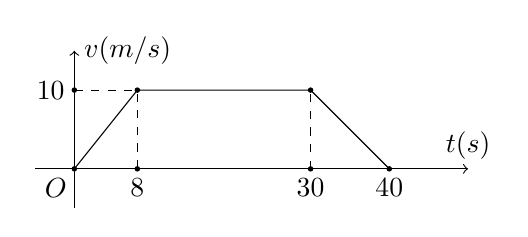
\begin{tikzpicture}
			\draw [->](-.5,0)node[below right]{$O$}--(5,0)node[above]{$t(s)$};
			\draw[->](0,-0.5)--(0,1.5)node[right]{$v(\text{m/s})$};
			\foreach \i /\t/\g in {(0,0),(0.8,0)/8/-90,(3,0)/30/-90,(4,0)/40/-90,(3,1)/ /0,(0.8,1)/ /0,(0,1)/10/180}{\fill \i circle(1pt);}
			\foreach \i /\t/\g in {(0.8,0)/8/-90,(3,0)/30/-90,(4,0)/40/-90,(3,1)/ /0,(0.8,1)/ /0}{	 \path \i node[below]{$\t$};}
			\path (0,1)node[left]{$10$};
			\draw (0,0)--(0.8,1)--(3,1)--(4,0);
			\draw[dashed](0,1)--(0.8,1)--(0.8,0) (3,0)--(3,1);
		\end{tikzpicture}
	\end{center}Quãng đường đi được (tính bằng m) của ca nô trong khoảng thời gian này là bao nhiêu?
	\shortans{$310$}
	\loigiai{
		Quãng đường đi được của ca nô trong $40$ giây là
			\begin{eqnarray*}
			S &=&
			\displaystyle\int\limits_{0}^{8} \dfrac{10}{8}x\mathrm{\,d}x+\displaystyle\int\limits_{8}^{30} 10\mathrm{\,d}x+\displaystyle\int\limits_{30}^{40} (-x+40)\mathrm{\,d}x\\
			&=&
			\dfrac{5x^2}{8}\bigg|_{0}^{8}+10x\bigg|_{8}^{30}+\left(-\dfrac{x^2}{2}+40x\right)\bigg|_{30}^{40}=310 \text{ m}.
		\end{eqnarray*}
	}
\end{ex}

\begin{ex}%[2H5H1-5]
	Trong không gian $Oxyz$, xét mặt sàn phẳng $(ABCD)$, với $A(1;1;0)$, $B(-2;3;-2)$, $C(0;0;-4)$, $D(3;-1;0)$. Tính khoảng cách từ điểm $E(8;1;2)$ đến mặt sàn $(ABCD)$.
	\shortans{$4$}
	\loigiai{
	Ta có $\vec{AB}=(-3;2;-2)$, $\vec{AC}=(-1;-1;-4)$.\\
	Gọi $\vec{n}$ là véc tơ pháp tuyến của mặt phẳng $(ABCD)$, suy ra \[\vec{n}=\left[\vec{AB},\vec{AC}\right]=(-10;-10;5)=-5(2;2;-1).\]
	Mặt phẳng $(ABCD)$ qua điểm $A$ và nhận $\vec{n'}=(2;2;-1)$ làm véc tơ pháp tuyến nên có phương trình là
	\[2x+2y-z-4=0.\]
	Khoảng cách từ $E$ đến mặt phẳng $(ABCD)$ là \[\mathrm{d}\left(E,(ABCD) \right)=\dfrac{\left|2\cdot 8 +2\cdot 1-2-4\right| }{\sqrt{2^2+2^2+(-1)^2}}=4.\] 
	}
\end{ex}

\begin{ex}%[2D4C3-2]
	\immini
	{Ông An xây dựng một sân bóng đá mini hình chữ nhật có chiều rộng $30$m và chiều dài $50$m. Để giảm bớt chi phí cho việc trồng cỏ nhân tạo, ông An chia sân bóng ra làm hai phần (tô đen và không tô đen) như hình bên. Phần tô đen gồm hai phần diện tích bằng nhau và đường cong $AIB$ là một parabol đỉnh $I$ được trồng cỏ nhân tạo với giá $130\,000$ đồng/m$^2$ và phần còn lại được trồng với giá $90\,000$ đồng/m$^2$. 
	}
	{\begin{tikzpicture}[scale=0.9, font=\footnotesize,line join=round, line cap=round, >=stealth]
			\coordinate (I) at (0,0);
			\coordinate (A) at (1.5,2.25);
			\coordinate (B) at ($(A)+(0,-4.5)$);
			\coordinate (C) at ($(B)+(-7.5,0)$);
			\coordinate (D) at ($(A)-(B)+(C)$);
			\coordinate (M) at ($(A)!1/2!(D)$);
			\coordinate (N) at ($(B)!1/2!(C)$);
			\coordinate (P) at ($(A)+(-1.5,0)$);
			\coordinate (Q) at ($(B)+(-1.5,0)$);
			\coordinate (R) at ($(D)+(1.5,0)$);
			\coordinate (S) at ($(C)+(1.5,0)$);
			\coordinate (td) at ($(D)+(0,0.3)$);
			\coordinate (dt) at ($(D)+(-0.3,0)$);
			\coordinate (ct) at ($(C)+(-0.3,0)$);
			\coordinate (tr) at ($(R)+(0,0.3)$);
			\coordinate (rp) at ($(R)+(0.3,0)$);
			\coordinate (I') at ($(R)!1/2!(S)$);
			\coordinate (g) at ($(I')+(0.3,0)$);
			\fill[gray]plot[domain=0:1.5](\x,{sqrt(3.375*(\x))})--(A)--plot[domain=1.5:0](\x,{-sqrt(3.375*(\x))})--cycle;
			\fill[gray](C)--(D)--plot[domain=-6:-4.5](\x,{sqrt(3.375*(-\x-4.5))})--plot[domain=-4.5:-6](\x,{-sqrt(3.375*(-\x-4.5))})--cycle;
			\draw (A)--(B)--(C)--(D)--cycle (M)--(N);
			\draw[dashed] (P)--(Q) (R)--(S);
			\draw[<->](td)--(tr);
			\node at ($(td)!1/2!(tr)$)[above]{$10$ m};
			\draw[<->](dt)--(ct);
			\node at ($(dt)!1/2!(ct)$)[above,rotate=90]{$30$ m};
			\draw[<->](rp)--(g);
			\node at ($(rp)!1/2!(g)$)[above,rotate=-90]{$15$ m};
			\foreach \x/\g in {A/90,B/-90,I/180,I'/-40}\draw[fill=black] (\x) circle (.05) +(\g:.5)node{\footnotesize$\x$};
	\end{tikzpicture}}
	\noindent
	Hỏi ông An phải trả bao nhiêu tiền (triệu đồng) để trồng cỏ nhân tạo cho sân bóng.
	\shortans{$151$}
	\loigiai{
		\immini{
			Chọn hệ trục tọa độ như hình vẽ ($I$ là gốc tọa độ). Khi đó đường cong $IAB$ là một parabol có phương trình dạng $y=ax^2$.\\
			Parabol đi qua điểm $\left(15;10 \right)$, suy ra 
			\[a \cdot 15^2=10 \Rightarrow a=\dfrac{2}{45}.\]
		}
		{
		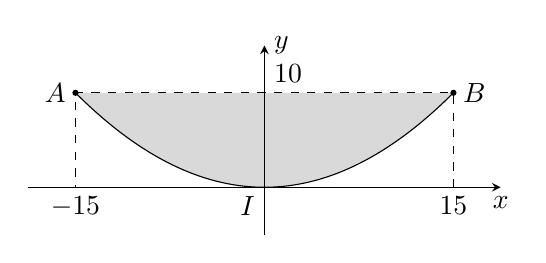
\begin{tikzpicture}[smooth,samples=300,scale=0.6,>=stealth]
			\fill[gray!30] (-4,2)--(4,2)--plot[domain=4:-4](\x,{0.125*(\x)^2});
			\draw[->] (-5,0)--(5,0) node[below]{$x$};
			\draw[->] (0,-1)--(0,3) node[right]{$y$};
			\draw (0,0) node[below left]{$I$};
			\draw[domain=-4:4] plot(\x,{0.125*(\x)^2});
			\draw[fill=black] (4,2) circle(1.5pt) (-4,2) circle(1.5pt);
			\draw[dashed] (4,0)node[below]{$15$}--(4,2)node[right]{$B$}--(-4,2)node[left]{$A$}--(-4,0)node[below]{$-15$};
			
			\node[right] at (0,2.4) {$10$};
	\end{tikzpicture}}
		\noindent
		Vậy $y=\dfrac{2}{45}x^2$. Diện tích phần tô đen là $S=2 \cdot \displaystyle\int\limits_{-15}^{15} \left(10-\dfrac{2}{45}x^2 \right) \mathrm{\,d}x=400 \, (\text{m}^2)$.\\
		Diện tích phần còn lại của sân bóng là $S_2=30 \cdot 50-400=1100\,(\text{m}^2).$\\
		Số tiền Ông An phải trả để trồng cỏ nhân tạo cho sân bóng là
		$$130000\times 400+90000\times 1100=151000000\text{ đồng}=151\text{ triệu đồng.}$$}
\end{ex}

\begin{ex}%[2H5C2-4]
	Trong không gian $Oxyz$, cho điểm $A(1;2;3)$ và hai đường thẳng
	\[d_1 \colon \dfrac{x-2}{2}= \dfrac{y+2}{-1}= \dfrac{z-3}{1},\quad d_2 \colon \heva{&x=1-t\\ &y=1+2t\\ &z=-1+t}\]
	Đường thẳng $\Delta$ qua $A$, vuông góc với $d_1$ và cắt $d_2$ tại $B$. Tính độ dài $AB$ (làm tròn đến hàng phần trăm).
	\shortans{$5{,}92$}
	\loigiai{
		Gọi $B=\Delta \cap d_2$, suy ra $B \in d_2$ nên $B(1-t;1+2t;-1+t)$.\\
		$d_1$ có vtcp $\vec{u}_1=(2;-1;1)$; $\Delta$ có vtcp $\vec{AB}=(-t;2t-1;t-4)$.\\
		Theo giả thiết, $\Delta \perp d_1$ nên $$\vec{AB}\cdot \vec{u}_1=0 \Leftrightarrow 2(-t)-1(2t-1)+(t-4)=0 \Leftrightarrow t=-1.$$
		Suy ra  $B(2;-1;-2)$. Độ dài đoạn thẳng $AB$ là
		$$AB=\sqrt{(2-1)^2+(-1-2)^2+(-2-3)^2}=\sqrt{35} \approx 5{,}92.$$	
	}
\end{ex}
\Closesolutionfile{ans}
\indapan{6}{ans/2GKII-DE2-3}